\documentclass{report}
% PAGE DIMENSIONS
\usepackage{geometry}
\geometry{a4paper,margin=3.5cm}

% PACKAGES
\usepackage[english]{babel}
\usepackage[T1]{fontenc}
\usepackage[utf8]{inputenc}
\usepackage{graphicx}
\usepackage{fancyhdr}
\usepackage{color}
\usepackage{eso-pic} %background pictures
\IfFileExists{inconsolata.sty}{\usepackage{inconsolata}}{}
\usepackage{csquotes}
\usepackage{booktabs}
\usepackage{tabularx}
\usepackage{array}
\usepackage{verbatim}
\usepackage{titlesec}
\usepackage{hyperref}
\usepackage{float}
\usepackage{caption}
\usepackage{subcaption}
\usepackage{amsmath,amsfonts,amssymb,amsthm}
\usepackage{xfrac}
\usepackage[intoc]{nomencl} %for abbreviations list
\usepackage{listings}
\usepackage{marginnote}
\usepackage{url}
\usepackage[normalem]{ulem}
\usepackage{tocbibind}
\usepackage{fancyhdr}
\usepackage{algorithm}
\usepackage{algpseudocode}

% Bibliography
\usepackage[style=numeric,natbib=true,sortcites=true,block=space,backend=bibtex]{biblatex}
\bibliography{ref/leonref,ref/kentref}
% Use 'biber %' to build bibliography

% Table of contents
\setcounter{tocdepth}{1}

% Headers and footers
\pagestyle{fancy}
\renewcommand{\headrulewidth}{0pt}
\lhead{\slshape \leftmark}
\chead{}
\rhead{}
\lfoot{}
\cfoot{}
\rfoot{\thepage}

% marginnote package options
\renewcommand*{\marginfont}{\color{red}\sffamily} %red, sans-serif
\reversemarginpar %margin notes on left side

% to justify typewriter monofont if used a lot in one place
\newcommand*\justify{%
  \fontdimen2\font=0.4em% interword space
  \fontdimen3\font=0.2em% interword stretch
  \fontdimen4\font=0.1em% interword shrink
  \fontdimen7\font=0.1em% extra space
  \hyphenchar\font=`\-% allowing hyphenation
}

% Define custom typewriter shorthands (uses \justify)
\newcommand{\justtt}[1]{\texttt{\justify{\small #1}}}
\newcommand{\smalltt}[1]{\texttt{{\small #1}}}

% listings package settings
\lstloadlanguages{Matlab,[ANSI]C}
\lstset{
  basicstyle=\ttfamily\small,
  %aboveskip=12pt,
  %belowskip=12pt,
  %frame=l,
  numbers=left,
  numberstyle=\ttfamily\tiny,
  numbersep=8pt,
  captionpos=b,
  tabsize=2,
  extendedchars=true,
  breaklines=true,
  showspaces=false,
  showtabs=false,
  keywordstyle=\color{blue},
  escapeinside={(*¤}{*¤)},
  %rangeprefix=,
  %rangesuffix=,
  includerangemarker=false,
  %stringstyle=\color{white}\ttfamily,
  %commentstyle=\color{white} %''cheat'' to hide comments
  xleftmargin=7pt,
  xrightmargin=7pt,
  %backgroundcolor=\color{lightgray},
  showstringspaces=false,
  morekeywords={}
}

% hyperref package settings
\hypersetup{
  unicode=true,          % non-Latin characters in Acrobat’s bookmarks
  pdftoolbar=true,        % show Acrobat’s toolbar?
  pdfmenubar=true,        % show Acrobat’s menu?
  pdffitwindow=false,     % window fit to page when opened
  pdfstartview={FitH},    % fit page to the window Horizontal/Vertical
  pdftitle={report},    % title
  pdfauthor={Kent Stark Olsen},% author
  pdfsubject={An analysis and implementation},   % subject of the document
  pdfkeywords= {University of Southern Denmark} {SDU}, % list of keywords
  pdfnewwindow=true,      % links in new window
  colorlinks=false,       % false: boxed links; true: colored links
  linkcolor=red,          % color of internal links
  citecolor=green,        % color of links to bibliography
  filecolor=magenta,      % color of file links
  urlcolor=cyan,           % color of external links
  plainpages=false
}

% Widow/orphan penalties
\widowpenalty=300
\clubpenalty=300

% \includegraphics default folder
\graphicspath{{graphics/}}

% Float positioning control
\setcounter{topnumber}{2}
\setcounter{bottomnumber}{2}
\setcounter{totalnumber}{3}
\renewcommand{\topfraction}{0.85}
\renewcommand{\bottomfraction}{0.85}
\renewcommand{\textfraction}{0.15}
\renewcommand{\floatpagefraction}{0.4}

% Header colour
\definecolor{FrontpageHeadingColor}{RGB}{5,5,60}%Heading colour definition

% Chapter name formatting
\titleformat
  {\chapter}%command
  [display]%shape
  {\normalfont\huge\bfseries}%format
  {\normalfont\Large\scshape\chaptertitlename\ \huge\thechapter}%label
  {10pt}%sep
  {\Huge}%before

% make nomenclature and change its heading/ text (see nomencl package)
\makenomenclature
\renewcommand{\nomname}{Abbreviations}
%
%  * Pass this line to MakeIndex:
%    %bm.nlo -s nomencl.ist -o %bm.nls
%
%  * Use \nomenclature{abbr}{discriptive text} to add an entry to the
%    abbreviations list (best done where the abbreviation first occurs in the text)
%  * Example:
%    \nomenclature{ADHD}{Attention Deficit Hyperactivity Disorder}

\begin{document}

% Front page
\pagenumbering{alpha} %frontpage numbered with a letter
\begin{titlepage}%
\currentpdfbookmark{Front page}{front_page}%hyperref pdf bookmark
\AddToShipoutPicture*{%background picture
 \put(0,0){
  \parbox[b][\paperheight][b]{\paperwidth}{%\parbox[position][height][inner-pos]{width}{text}
   \vfill
   %\begin{flushright}
   
\includegraphics[width=0.43\paperwidth,trim=110 0 0 0]{content/00_frontmatter/sdu_seal.pdf}%trim=l b r t
   %\end{flushright}
   \vspace*{2.9cm}
  }
 }
}
\begin{flushright}

\includegraphics[scale=0.73]{content/00_frontmatter/sdu_logo.pdf}
\end{flushright}
\vspace*{2.7cm}
\setlength{\extrarowheight}{0pt}
\textsf{\Huge{\textbf{\textcolor{FrontpageHeadingColor}{Hand-eye calibration}}}}\\
\vspace*{0.5cm}
\textsf{\Large{\textbf{\textcolor{FrontpageHeadingColor}{for an eye-in-hand 3D reconstruction system}}}}\\
\vspace{1.0cm}
\setlength{\extrarowheight}{1.5pt}
\begin{tabular}{@{}l l}
	\textsf{\large{Participants}} & \textsf{\large{Frederik Hagelskjær, M.Sc. student, Robot Systems Engineering}}\\
	& \textsf{\large{The Maersk Mc-Kinney Moller Institute}}\\
	\\
	& \textsf{\large{Kent Stark Olsen, M.Sc. student, Robot Systems Engineering}}\\
	& \textsf{\large{The Maersk Mc-Kinney Moller Institute}}\\
	\\
	& \textsf{\large{Leon Bonde Larsen, M.Sc. student, Robot Systems Engineering}}\\
	& \textsf{\large{The Maersk Mc-Kinney Moller Institute}}\\
	\\
	& \textsf{\large{Rudi Hansen, M.Sc. student, Robot Systems Engineering}}\\
	& \textsf{\large{The Maersk Mc-Kinney Moller Institute}}\\
	\\
	\textsf{\large{Computer Vision Supervisor}} & \textsf{\large{Dirk Kraft, Associate Professor}}\\
	& \textsf{\large{The Maersk Mc-Kinney Moller Institute}}\\
	\\
	\textsf{\large{Robotics Supervisor}} & \textsf{\large{Lars-Peter Ellekilde, Associate professor}}\\
	& \textsf{\large{The Maersk Mc-Kinney Moller Institute}}\\
	\\
	\textsf{\large{ECTS}} & \textsf{\large{10}}\\
	\\
	\textsf{\large{Period}} & \textsf{\large{Spring 2014}}
\end{tabular}
\vfill
\textsf{\\Faculty of Engineering\\
University of Southern Denmark\\
Niels Bohrs Allé 1\\
5230 Odense M\\
Denmark}
\vspace*{10pt}
\\
\textsf{www.sdu.dk/tek\\
+45 6550 7303\\
tek@tek.sdu.dk}
\end{titlepage}

% Abstract (un-numbered chapter)
\pagenumbering{roman} %until main content we use roman page numbering
\chapter*{Abstract}\addcontentsline{toc}{chapter}{Abstract}
Digital representations of three-dimensional objects are of great importance to many applications. Often the 3D models are hand-build which can be a tedious and time consuming task thus making automatic modelling desirable. In robotics, models of the environment are used as a priori knowledge for collision checking. The problem with hand-build models is that they limit the application of robots to known environments. \\

One method for recording 3D models is to mount a stereo camera on the end effector of a robot arm (eye-in-hand) and let the robot move the camera to the views needed to generate the model. This way the robot is able to assess unknown objects and update the work cell model accordingly. In this work we propose a calibration method based on point clouds and we present a fully functional system based on ROS and build from scratch. Development of the system was aimed at investigating the hypothesis that a locally calibrated system could generate significantly better models than the same system without calibration and that basing the entire system on the ROS framework would reduce development time. \\

Evaluation of the system was based on a comparison between the hand-eye calibration module implemented in ROS and the proposed application specific calibration. Although several experiments were made, they mostly served to get acquainted with the system and the results are insufficient to draw any final conclusions, but, some partial conclusions are stated. The calibration method worked, but performed poorly and can thus not be recommended at this point. The implementation of the system in ROS based on the environment interaction model worked well. \\

% Preface (un-numbered chapter)
\chapter*{Preface}\addcontentsline{toc}{chapter}{Preface}
Preface my ass...

% Table of contents, figures, tables, listings and abbreviations
\tableofcontents
%\listoffigures
%\listoftables
%\lstlistoflistings\addcontentsline{toc}{chapter}{Listings}
%\printnomenclature[1.5cm]

% MAIN CONTENT
%\clearpage
\pagenumbering{arabic} %''normal'' arabic numbering from here on out
\chapter{Introduction}
Digital representations of three-dimensional objects are of great importance to many applications. Often the 3D models are hand-build which can be a tedious and time consuming task thus making automatic modelling desirable. In robotics, models of the environment are used as a priori knowledge for collision checking. The problem with hand-build models is that they limit the application of robots to known environments. \\

One method for recording 3D models is to mount a stereo camera on the end effector of a robot arm (eye-in-hand) and let the robot move the camera to the views needed to generate the model. This way the robot is able to assess unknown objects and update the work cell model accordingly. The precision of the model is not only dependent on the quality of robot arm and camera, but also on the calibration of the system. The camera can be calibrated using a marker plate in different poses thus calculating intrinsic and extrinsic parameters for the camera \cite{Zhang2000}. The system can be further calibrated in a process called hand-eye calibration solving for the unknown spatial relationships in the kinematic chain.\\

%Another important part of 3D modelling is the reconstruction problem, reasoning about either surface, volume or both. Depending on the application there are very different demands for the final model. If it is used for collision detection a coarse model is more efficient, while a model for grasping needs to be sufficiently detailed to infer grasping points. Modelling is a multi-step process where the gathered data is first transformed, filtered and combined to form a point cloud representing the object. Next an indicator function is approximated to best fit the normals of the inferred solid. Finally a mesh is generated from the indicator function. Using wavelets to approximate the indicator function provides a localised, multi-resolution representation and thus addresses the trade-off between faster coarse models and slower fine models.\\

Normally the hand-eye calibration is performed based on images capturing a marker plate from different angles. Features matched between the images are then used to formulate a set of equations to solve for the unknown transforms from end-effector to camera and from robot base to the object. In this work, another approach is suggested, performing the calibration based on point clouds obtained from capturing the object. There are several advantages of this, but most importantly the process can be fully integrated in the robots behaviour, since it does not require a special calibration marker and the system can be calibrated locally, thus potentially increasing the accuracy.\\

\textit{It is hypothesised that a locally calibrated system can generate significantly better models than the same system without calibration and that basing the entire system on the ROS framework will reduce development time.} \\

The calibration is evaluated in a manipulative study, where a known object is modelled before and after calibrating the system. The produced point clouds are visually as well as quantitatively compared to the true 3D model of the object. The novelties in this report are hand-eye calibration based on point cloud data and implementing the entire system in Robot Operating System(ROS).\\

In chapter 2 the system is analysed on component level to formulate a requirements specification forming the basis for chapter 3 describing decision making, chapter 4 describing robotics, chapter 5 describing computer vision and chapter 6 describing 3D modelling. Chapter 7 presents the proposed point cloud based calibration system and finally in chapter 8 the evaluation method and findings are presented and discussed, leading to a conclusion in chapter 9.

% Analysis
\chapter{Analysis}
The system must be capable of performing 3D reconstruction based on the eye-in-hand principle, meaning that a stereo camera is mounted at the end-effector of a robot arm. Implementation of the system must be based on the Robot Operating System (ROS) as this is the controller interface for both robot and sensors. The architecture of the system(Figure \ref{fig:block_diagram}) is a closed loop structure based on the Good Old Fashion Artificial Intelligence(GOFAI) environment interaction model \cite{Pfeifer2007a}. In the following each part of the system will be analysed with respect to functionality and responsibilities leading to a formulation of a requirements specification.

\begin{figure}[htb]
	\begin{center}
		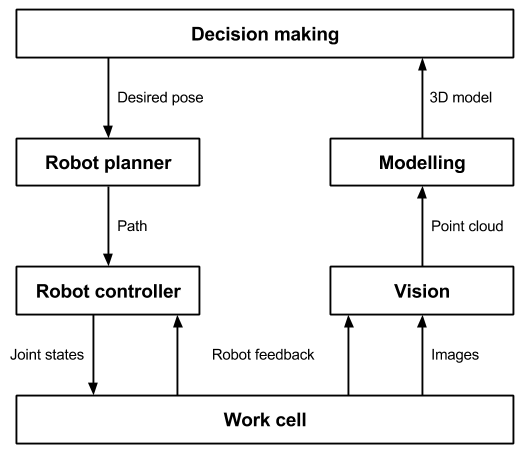
\includegraphics[scale=0.5,trim=0 0 0 0]{graphics/02_analysis/block_diagram.png}%trim=l b r t
		\caption{Block diagram of the eye-in-hand 3D reconstruction system.}
		\label{fig:block_diagram}
	\end{center}
\end{figure}

\subsection{Decision maker}
The decision maker is the highest level of abstraction and authority in the system and is responsible for controlling the task, which in this case means moving the robot arm to the right poses and capture images from the sensor. The task can be broken down to starting the process, choosing a pose, executing the pose, capturing the image and ending the task when there are no more poses needed. Any further work like next best view planning, automatic calibration or other alternative tasks will be implemented in the decision maker and it should therefore be general and easy to expand. In the current application, the desired poses will be generated to capture the object from a number of discrete locations on a sphere subject to distance and viewpoint constraints. The captions must be evenly distributed to cover the entire object. 

\marginnote{Errors...} 


\subsection{Robot planner}
The robot planner is the top level abstraction of the robot arm and takes desired pose in 3D space as input generating a desired path in joint space as output. It is responsible for generating the path between the current pose of the robot and the desired pose. The path is subject to a number of physical constraints and must therefore be generated in steps. The first step is to find a collision free path through the workspace thus requiring a kinematic model of the robot as well as a priori 3D models of robot and work cell. When a suitable path has been found, the path must be optimised for length, clearance and undesired movement. In cases where a collision free path cannot be found, the robot planner must relay this back to the decision maker. Implementations in the robot planner must be robust and therefore make use of some of the widely used open source libraries and ROS stacks should be facilitated. 

\subsection{Robot controller}
The robot controller executes the path and thus handles communication to low level controllers and feedback sensors on the robot. The path is executed in a closed-loop control system and therefore the joint states realising the path must be converted to actuator velocities. This is done by adding a time dimension to the path, subject to joint velocity constraints. The time tessellated path is further blended to meet acceleration and jerk constraints and is finally interpolated and executed in the control loop. Implementations should be robust and therefore make use of some of the many open source libraries and ROS stacks. 

\subsection{Work cell}
The workcell contains a six degrees of freedom RX60 robot arm with a bumblebee stereo camera and a carmine sensor mounted on the end effector(Figure \ref{fig:block_diagram}). The work cell interface is based on a ROS node communicating with the physical robot controller and a node broadcasting data from the camera. Since the RX60 has limited reach, the objects being modelled are hanged from a point over the robot. The a priori model of the work cell contains only the robot arm and simplified bounding boxes representing the immediate surroundings of the robot. 

\marginnote{Image missing}
%\begin{figure}[htb]
%	\begin{center}
%		\includegraphics[scale=0.5,trim=0 0 0 0]{graphics/02_analysis/work_cell.png}%trim=l b r t
%		\caption{The work cell containing RX60 robot mounted with stereo camera.}
%		\label{fig:work_cell}
%	\end{center}
%\end{figure}

\subsection{Vision}
The vision module takes input from the stereo camera mounted on the end effector of the robot and from that generates a 3D point cloud. The images are undistorted and rectified using calibration parameters obtained independently of the system using the ROS calibration node. When the robot is at rest in the desired pose, a signal from the decision maker tells the vision component to capture the two images from the sensor. From the two images a disparity image is formed and by using the obtained projective parameters the point cloud is generated. Implementation should be based on ROS packages and the OpenCV library for image processing.

\subsection{Modelling}
The Modelling part takes point clouds as input and these are transformed to a common frame based on the absolute pose from which they were recorded and a relative pose estimated from matching the points. The combined point cloud is then cropped and filtered to be ready for 3D surface reconstruction. The reconstruction process is performed offline and produces 3D models.

\subsection{Calibration}
The calibration process is responsible for calibrating the system prior to running the task. There are numerous sources of errors in the system, but in a closed-loop system thorough calibration can limit the effects of inaccuracies. Performing a hand-eye calibration can provide the exact transform between camera view and the end-effector, thus in theory removing the need for relative pose estimation in combining the point clouds.


\subsection{Requirements specification}
The above analysis leads to a requirements specification (Table \ref{tab:requirements}) for the combined system.

\begin{table}
	\label{tab:requirements}
	\caption{Requirements specification}
    \begin{tabular}{|l|l|l|}
    \hline
    Block            & Component      & Requirements                                       \\ \noalign{\hrule height 2pt}
    Decision maker   & Pose generator & poses on an equidistant sphere                     \\ \hline
    ~                & ~              & viewpoint at the object                            \\ \hline
    ~                & ~              & evenly distributed                                 \\ \hline
    ~                & State machine  & choose pose                                        \\ \hline
    ~                & ~              & ready for capture signal                           \\ \hline
    ~                & Error handler  & handle impossible pose                             \\ \noalign{\hrule height 2pt}
    Robot planner    & Detector       & detect self collision                              \\ \hline
    ~                & ~              & detect work cell collision                         \\ \hline
    ~                & Planner        & find collision free path                           \\ \hline
    ~                & Optimisation   & optimise path length                               \\ \hline
    ~                & ~              & optimise clearance                                 \\ \hline
    ~                & ~              & remove undesired movement                          \\ \hline
    ~                & Model          & forward kinematics                                 \\ \hline
    ~                & ~              & inverse kinematics                                 \\ \hline
    ~                & ~              & joint limits                                       \\ \noalign{\hrule height 2pt}
    Robot controller & Blender        & tessellation in time                               \\ \hline
    ~                & ~              & handle velocity, acceleration and jerk constraints \\ \hline
    ~                & Control        & get feedback                                       \\ \hline
    ~                & ~              & interpolate path                                   \\ \hline
    ~                & ~              & closed loop control                                \\ \hline
    ~                & Communication  & set joint angles                                   \\ \hline
    ~                & ~              & get joint angles                                   \\ \noalign{\hrule height 2pt}
    Work cell        & Objects        & hang from above the robot                          \\ \hline
    ~                & ~              & known model of objects                             \\ \hline
    ~                & Interface      & ROS based                                          \\ \noalign{\hrule height 2pt}
    Vision           & Camera         & ROS interface                                      \\ \hline
    ~                & ~              & calibration for intrinsic parameters               \\ \hline
    ~                & ~              & calibration for projective parameters              \\ \hline
    ~                & Preprocessor   & undistortion                                       \\ \hline
    ~                & ~              & rectification                                      \\ \hline
    ~                & Controller     & capture images when signaled                       \\ \hline
    ~                & Processor      & generate disparity image                           \\ \hline
    ~                & ~              & generate point cloud                               \\ \noalign{\hrule height 2pt}
    Modelling        & Filtering      & transform points to common frame                   \\ \hline
    ~                & ~              & downsample                                         \\ \hline
    ~                & ~              & combine point clouds                               \\ \hline
    ~                & Reconstruction & generate surface                                   \\ \hline
    \end{tabular}
\end{table}


% Decision making
\chapter{Decision making}
The decision making component generates 8 poses evenly distributed on an sphere of radius 0.5 meters, always with the viewpoint at the center of the sphere. As the object is not static in the scene, the center of the sphere can be moved by an interactive marker as shown on figure \ref{fig:robot_moving_around_object}. The poses are executed by the planner, and when the desired pose has been reached a message is be passed to the sensor nodes to do a capture.


\begin{figure}[htb]
	\begin{center}
		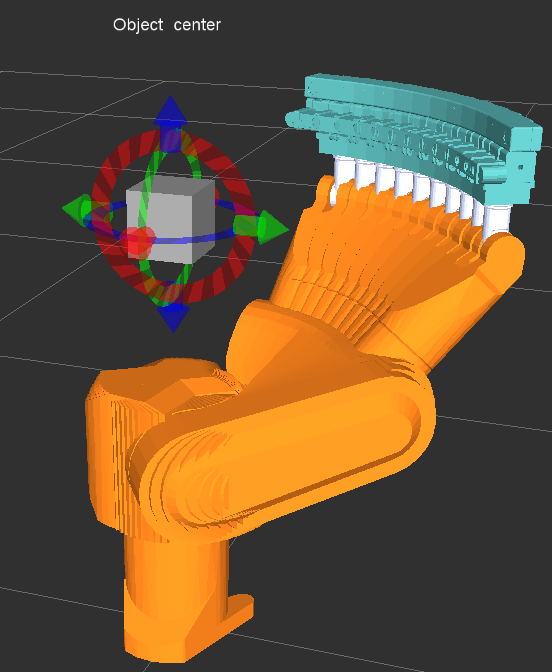
\includegraphics[scale=0.5,trim=0 0 0 0]{graphics/04_decisionmaking/robot_moving_around_object.png}%trim=l b r t
		\caption{The spin center is moveable by an interactive marker. The robot has planned a path to the next desired pose}
		\label{fig:robot_moving_around_object}
	\end{center}
\end{figure}

%\subsection{SMACH}
%SMACH = Next best view ready code
%state machine diagram?

\subsection{Special message type}
For easy offline manipulation of data a messagetype has been defined to carry the information acquired at each pose. Using this format allows the data to be captured at one point in time and processing at another by using rosbag between the nodes. Initially the message only contains the pose id, max number of poses and poses of the sensors, it is then passed on to the stereo camera node where the captured images are appended. Afterwards the dense\_stereo node creates and appends 3D information from the captured images and finally it can be passed to the reconstruction node.

\begin{figure}[htb]
	\begin{center}
		
\includegraphics[scale=0.5,trim=0 50 0 0]{graphics/04_decisionmaking/message_path.png}%trim=l b r t
		\caption{The path of the message between the related nodes in the system. In each node new data is appended}
		\label{fig:message_path}
	\end{center}
\end{figure}

\subsection{State Machine}
The task is performed as a state machine (Figure \ref{fig:state_diagram}) consisting of two main states, move and capture. The move state executes a list of poses by issuing one pose at a time to the robot planner and wait for the robot state to reach within a threshold of the desired pose. Arriving at the pose transitions the state machine into the capture state, signalling the sensor node to collect data. Based on a time delay, the capture state transitions back to the move state. When the list of poses has all been executed, the move state remains at the final pose.


\begin{figure}[htb]
	\begin{center}
		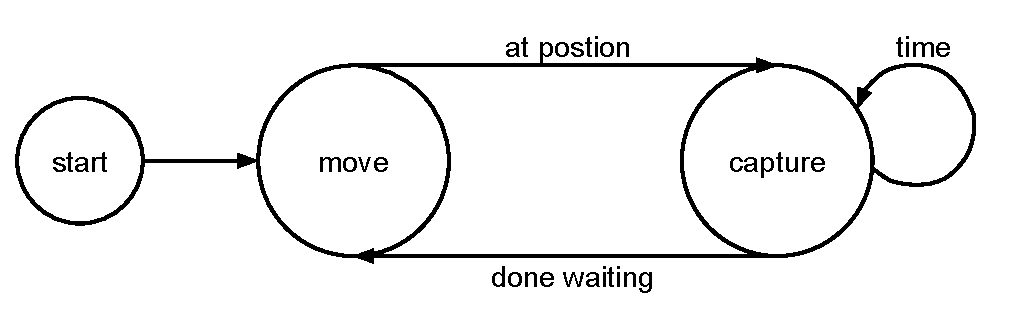
\includegraphics[scale=0.5,trim=0 0 0 0]{graphics/04_decisionmaking/state_diagram.pdf}%trim=l b r t
		\caption{State diagram of the decision maker}
		\label{fig:state_diagram}
	\end{center}
\end{figure}


% Robotics
\chapter{Robotics}
\marginnote{Needs to be refering more to the project requirements}.

This chapter describes the setup of the robot system used with the focus of making a quick reference for fast setting up a robot system using tool in the ROS framework. The task of the robot in this project is to be able to move the camera sensor around the object to capture images from different poses. For this purpose a 6 axis Stäubli rx60 has been provided along with a ROS service interface to query and control the configuration. The robot and workcell will be descried in further details in section \ref{sec:robot_physical}. For the robot to be able to move from one pose to another, planners, collision checking and controllers are needed. For the planner to be able to do the collision checking without actually colliding, a model of the robot and the workcell must be present. How to setup this model and available parameters are shortly descriped in section \ref{sec:robot_model}. Planning a collision free path is done with ROS MoveIt. ROS Control is used to make the interface between MoveIt and the robot. The MoveIt concepts and how to set it up is described in section \ref{sec:moveit}, a further look in to the planning\marginnote{Skipped} algorihtms in section \ref{sec:planning} and a short introduction to ROS control in section \ref{sec:robot_control}. A graphical overview of the system is given in figure \ref{fig:workcell_to_moveit_path}

\begin{figure}[htb]
	\begin{center}
		
\includegraphics[scale=0.5,trim=0 0 0 0]{graphics/05_robotics/workcell_to_moveIt_path.png}%trim=l b r t
		\caption{Overview of the path from the workcell to the MoveIt stack}
		\label{fig:workcell_to_moveit_path}
	\end{center}
\end{figure}

% Remember to refer the requirement specification, give a breif introduction to why MoveIt has been used and also a short abstact of what this chaper contains.

% General overview of the system

\section{The physical robot and ROS interface}
\label{sec:robot_physical}
% - Staübli (boot up)
The robot provided for this project is a Stäubli RX60b 6 Axis industrial manipulator. When starting the robot a small rotary switch at the bottom of the controller needs to be turned, and after a few minutes the robot will be booted up and ready. Interfacing the robot is done by a small teach pendant, where it is possible to change application, calibrate, manual control etc. For this project a robot application has been provided such that the robot communicates with a ROS node on a provided machine thus almost no interfacing directly with the robot is necessary. When starting the robot it needs to run the robot application, which is done by releasing the emergency stop, pushing the big green button i the top right corner so it lids up and pressing the (un)pause button. When doing tests with the robot it can be recommended to adjust the moving speed to a minimum to avoid accidents. This is done by the plus and minus buttons on the pendant.
% - The tool unit and sensors (breif)
The tool mounted on the tool flange is a 3D printet sensor mount with both a Carmine depth camera and a PointGrey BumbleBee stereo camera. Wires have been strip mounted to the robot to avoid them getting stuck in the moving parts. 
% - Workcell
The workcell contains the robot placed on plane big surface, a Troax safety fence and a radiator. Both the fence and the radiator is placed in such distance that the robot will only be able to collide with them in very few configurations. The workcell can be seen in figure \marginnote{Image missing}.

% ------------------------------------------- PICTURE OF ROBOT AND WORKCELL ---------------------------------------

% - The ROS service interface
The robot axis are controlled by the robot controller which are then connected to a computer with a provided ROS application for communication. To control the robot service calls needs to be made to this node. These service calls provides functionality such as setting various limits, tool position, valve control and most important joint configurations. Furthermore it allows values to be read from the robot, such that feedback to the trajectory controller can be supplied.

\section{Robot model}
\label{sec:robot_model}
To be able to plan a trajectory for the robot, the planner needs a model of the robot. This model is used both for kinematics but also to avoid self collision. The format for describing a robot in ROS is Unified Robot Description Format (URDF). It is also possible to define the robot in the XACRO macro format and convert it to the macro language URDF, however in this project the robot has been descried directly in URDF.
% - URDF format and tools (can also be used in gazebo)
A tool that can be used to generate the URDF file directly from a CAD assembly file is available under the name "SolidWorks to URDF Exporter". This tool was used as a basis for the URDF file for this project, but the quality of the output is somehow questionable. A RobWork workcell containing the description of the RX60 robot was available for the project and has been used as a reference to describe the joints, joints limits and also as source for robot CAD files. It needs to be noticed that CAD format has to be binary STL to work as part of the robot description. The tool on the robot has also been described in the URDF to give the necessary transforms for the camera sensors and a intuitive looking visualization of the robot. In the URDF file it is possible to define both a visual CAD of the joints but also a CAD only used for collision checking. To be sure that the tool does not collide with anything, the collision model is a large box with a least 10mm extra space margin with respect to the visual model. The model can be seen on figure \ref{fig:tool_collision_model}. To use the URDF file it has to be put into the parameter server which can be done in the launch file \marginnote{Needs explaning?}.

\begin{figure}[htb]
	\begin{center}
		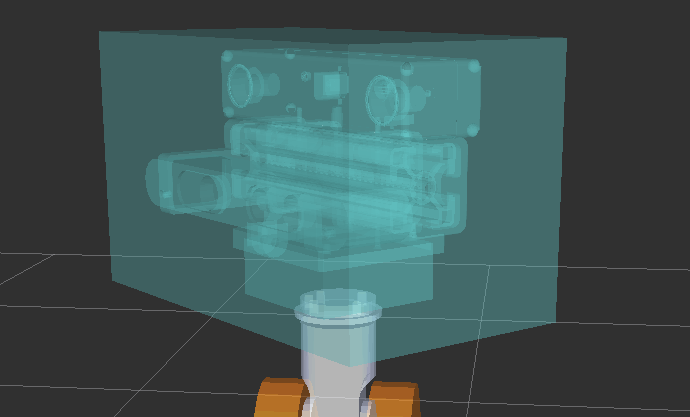
\includegraphics[scale=0.5,trim=0 0 0 0]{graphics/05_robotics/tool_collision_model.png}%trim=l b r t
		\caption{The tool mounted on the robot flange and the collision model shown in transparent}
		\label{fig:tool_collision_model}
	\end{center}
\end{figure}

% - - Collision model and visual model
% - TF tree
% - Visualization
\section{ROS MoveIt}
\label{sec:moveit}
ROS MoveIt is a software planing tool that collect many opensource libraries to a tool that can easily be used for planning with both simple and high dimensionality robots. A great example of a complex robot is the PR2 robot developed at Willow Garage that runs on MoveIt.
Controlling a robot with MoveIt can be done by the C++ or python interface, but it also features a planning plugin for the ROS visualizer (Rviz). Combining the programming interface with Rviz gives a great visual feedback, where the planned trajectory can be visualized before and while moving the robot as seen on figure \ref{fig:robot_trajectory}.

\begin{figure}[htb]
	\begin{center}
		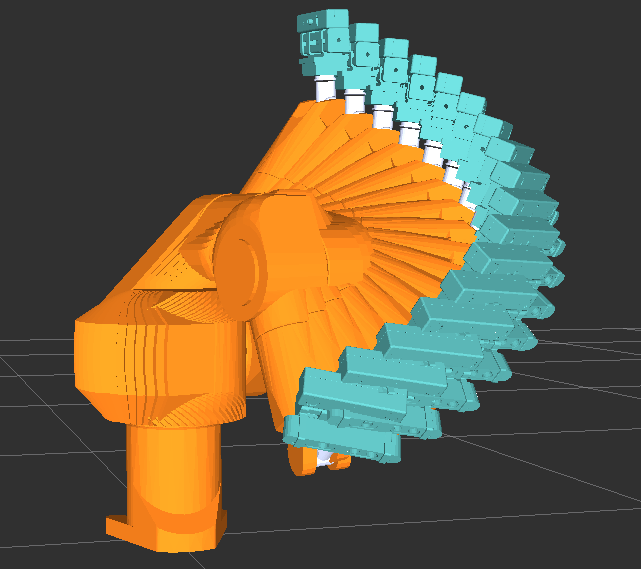
\includegraphics[scale=0.5,trim=0 0 0 0]{graphics/05_robotics/robot_trajectory.png}%trim=l b r t
		\caption{Robot trajectory displayed as a series of robot configurations in Rviz}
		\label{fig:robot_trajectory}
	\end{center}
\end{figure}

When planning in MoveIt it will by default use the Open Motion Planneing Library (OMPL), however MoveIt provides a plugin interface allowing custom planners to be used. OMPL is a collection of state of art sample based planners that takes a planning request and collision detector as input and if successful returns a planned path. MoveIt then generate a trajectory from the path according to the given robot constraints. The collision checking in MoveIt is done by Flexible Collision Library (FCL). This collision detection allows different input models, such as robot self-collision, workcell model collision and collision with sensed objects. For collision with sensed data, MoveIt has a self-filter, such that if a part of the robot is sensed it can be filtered away from collision map. Without this feature, the sensed robot would collide with the kinematic calculated position of the robot. As default MoveIt uses Orocos KDL for solving the kinematics, but for complex robots it is recommended to compile a robot specific solver using OpenRave IKfast.

% - Features / introduction
% - - Support for octomap input for collsion checking with self-filter (removes visible parts of the robot from the map)
% - - OMPL - Motion planning (OMPL itself has no concept of a robot)
% - - OpenRave IKFast - Kinematic solver / Orocos KDL
% - - FCL - Collision checking
% - Importing the robot (robot setup tool)
% - Interfaces (rviz, c++, trajectory service)
% - - rviz, c++
% - - controller manager (trajectory action interface)
% - Constrainting the robot

% - Robot state publisher (TF)
%\section{Planning}
%\label{sec:planning}
% - PRM planner
% - Path optimization
% - How is it done in OMPL?
\section{Robot control}
\label{sec:robot_control}
% - ROS Control framework

%Motion planning
%  general motion planning, kinematics
%  Available tools in ROS
%  MoveIt planner concepts
%  Setting up a new robot with MoveIt
%  Robot model (URDF (joints, links, limits, transforms) , CAD, rviz/TF)
%Robot controller
%
%C++ planning interface


% Vision
\chapter{Vision}


This chapter covers the transformation of 2D stereo images into a useful 3D point cloud. Using only a stereo camera as passive sensor.

\section{Theory - Dense Stereo}

Dense stereo uses two 2D images and converts them to a dense 3D point cloud. That is the 3D postion of every point in the 2D images is desired. To obtain this the disparity between all features are required, and the following stages are done with that in mind. The stages are as following.

\begin{itemize}
  \item Undistortion
  \item Rectification
  \item Correspondence
  \item Reprojection
\end{itemize}


\subsection{Undistortion and Rectification}


The undistortion and rectification are performed automatically and therefore only a short description will be included. By knowledge of these parameters one could make functions take them into account, but it is much more effective to transform the images.

As a lens is used for the cameras the pin hole camera model cannot be used, i.e. a 3D point, X, is mapped to the image plane, x, by $ x = f X/Z $, where f is the focal length and Z is the distance to the camera. Both radial and tangential distortion exist respectively creating the circular and elliptical distortion. By correcting the image for these parameters all pixels now follow the camera model and their projection line can be found.

The basic idea of rectification is based on epipolar lines. Epipolar lines are created by knowing the transform between the cameras. For every single point in one camera the line on which it can appear on another camera can be found. That is the epipolar line is a mapping of a pixels projection line in one camera onto the image plane of another camera. 

By knowing the transformation between the two images, epipolar lines can be created for every point. An epipolar line is the line on which any point in one image must be positioned in the other image. Thus making the search for a feature much faster as it only occurs in one dimension.

Rectification takes this one step further. By rectifying the two images the camera planes are angled towards the baseline, thus being parallel. Making the search for correspondence a 1D horizontal task, drastically increasing the speed.

Thus undistortion is a manipulation done independently for the cameras and the rectification is performed for the two cameras together, using respectively the intrinsic and extrinsic parameter.


\subsection{Correspondence} \label{sec:correspondence}

Correspondence is the matching pixels position in different images. This creates a disparity map for all pixels in the images. Though there is no guarantee that the disparity map is actually correct. 

The main goal in dense stereo can be described as minimizing the global error. 

Most of the top-ranked algorithms for the Middlesbury Stereo vision comparison use global optimization \cite{Hirschmuller2008}. Global optimization tries to minimize the overall error in the disparity image, i.e. creating the optimal disparity image. Though as this is an NP-hard problem for the sake of speed these where not considered.

The opposite approach is a horizontal 1D scan. As the rectification of the images guarantees horizontal epipolar lines, the most simple approach would be a 1D scan optimized for the lowest error. The problem is that a single scanline algorithm would lead to a very low vertical consistency of disparity. 

Instead a semi global approach is used as a compromise between the two methods. 

The idea of the semi global matching is an optimization of the disparity locally, but consistent. Following equation \ref{eq:cost} the penalty for small changes and large changes are distinguished as respectively $P_{1}$ and $P_{2}$. Here C is the pixel wise matching cost for disparity $D_{\textbf{p}}$ at position \textbf{p} and \textbf{q} is nearby positions.

\begin{equation}\label{eq:cost}
\begin{split}
E(D) = \sum\limits_{\textbf{p}}(C(\textbf{p},D_{\textbf{p}}) + \sum\limits_{\textbf{q} \in N_{\textbf{p}} } P_{1} T [|D_{\textbf{p}} - D_{\textbf{q}}| = 1] + \sum\limits_{\textbf{q} \in N_{\textbf{p}} } P_{2} T [|D_{\textbf{p}} - D_{\textbf{q}}| > 1]
\end{split}
\end{equation} 

The optimization is then done as a shortest path for multiple 1D paths. Figure \ref{fig:paths} shows an example of this using 16 paths, in the actual implementation only 5 paths are used for the sake of speed. A disparity range for which the path is found is defined beforehand, thus a limit is set to which disparity’s can be found. 

\begin{figure}[h!]
  \centering
    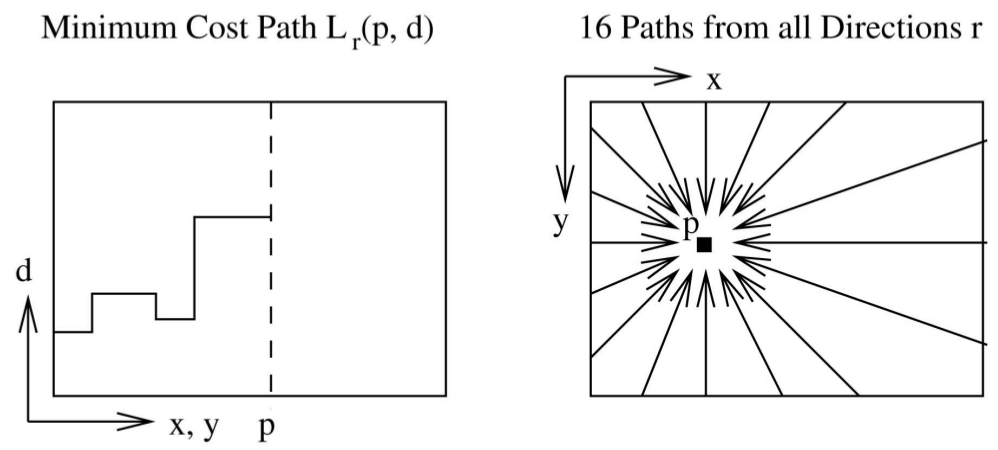
\includegraphics[scale=0.2]{graphics/06_vision/cost_aggregation.jpg}
      \caption{Costs for all directions are calculated using specific disparities and the disparity with the shortest path is found.}
    \label{fig:paths}
\end{figure}

Mutual information \cite{egnal2000mutual} is used as the pixelwise matching. Using mutual information makes the algorithm much better at handling handling radiometric distances. The mutual information needs the disparity map to calculate the pixel matching cost, $ C_{MI} $. Because of that the algorithm starts with a downscaled disparity guess and consistently runs through and upscales until it reaches full size. 


Consistency check is performed as in equation \ref{eq:consistency} using both disparity images. This removes errors that were created by occlusion in any of the images. Thus if the disparities differ they are set to invalid. 

\begin{equation}\label{eq:consistency}
\begin{split}
D_{p} =  
\begin{pmatrix}
	D_{bp}	&  if|D_{bp} - D_{mq}| \leq 1, \\
	D_{inv} & otherwise
 \end{pmatrix}
\end{split}
\end{equation} 

%\begin{equation}\label{eq:qdefinition}
% \begin{split}
%  q = e_{bm}(p,D_{bp}) 
% \end{split}
%\end{equation} 

The flowchart of the complete system as described in the original article \cite{Hirschmuller2008} can be seen in figure \ref{fig:complete_system}.


\begin{figure}[h!]
  \centering
    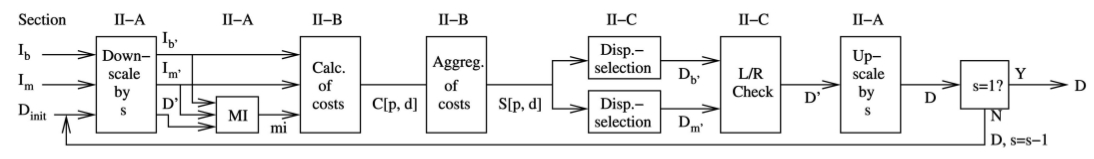
\includegraphics[width=\textwidth]{graphics/06_vision/complete_system.jpg}
     \caption{ Flowchart of the complete stereo process for SGBM. } 
    \label{fig:complete_system}
\end{figure}


\subsection{Reprojection} \label{sec:reprojection}

During the calibration of the cameras, projection matrices were obtained for both cameras. The projection matrices are based on the left camera lens, meaning the baseline, distance to the left camera, is 0 for the left matrix. By multiplying the projection matrix with a 3D point in the left cameras coordinate system, the points position in the image can be found as in equation \ref{eq:projection}. 


\begin{equation}\label{eq:projection}
 \begin{split}
  \begin{pmatrix}
   x \\
   y \\
   \omega 
  \end{pmatrix}	
  = 
  \begin{pmatrix}
    F_{x} & 0 & C_{x} & -F_{x}T_{x} \\
    0 & F_{y} & C_{y} & 0 \\
    0 & 0 & 1 & 0
  \end{pmatrix}
  \begin{pmatrix}
   X \\
   Y \\
   Z \\
   1 
  \end{pmatrix}	
 \end{split}
\end{equation}  


Here $F_{x}$ and $F_{y}$ are the focal length of the camera, $C_{x}$ and $C_{y}$ are the middle position of the image.

$T_{x}$ is the translation to the left camera. That is for the right camera it is the baseline and for the left it is 0. The baseline is measured in millimetres. 

But the goal is to obtain the opposite, the transform from 2D to 3D. That is the action of converting the obtained disparity map into a 3D point cloud. To do that the x and y positions are combined with the disparity. Thus multiplying with the Q matrix the 3D map position can be found.

\[ Q [ x \ y \ d \ 1 ]^{T} = [ X \ Y \ Z \ W ]^{T} \]

Where the Q matrix is defined by the parameters in the right projection matrix, except for the $C_{x}'$.

\[
Q =
 \begin{pmatrix}
  1 & 0 & 0 & -C_{x} \\
  0 & 1 & 0 & -C_{y} \\
  0 & 0 & 0 & F_{x} \\
  0 & 0 & -1/T_{x} & (C_{x}-C_{x}')/T_{x} 
 \end{pmatrix}
\]

Thus multiplying with the above mentioned vector, and scaling W to one the 3D position can be obtained.

\[
 \begin{pmatrix}
  x - C_{x} \\
  y - C_{y} \\
  F_{x} \\
  d-1/T_{x} 
 \end{pmatrix}
 \Rightarrow
  \begin{pmatrix}  
  X\\
  Y\\
  Z
 \end{pmatrix}
 =
 \begin{pmatrix}
  \dfrac{x - C_{x}}{ d(-1/T_{x})}  \\
  \dfrac{y - C_{y} }{ d(-1/T_{x})}\\
  \dfrac{F_{x}}{ d(-1/T_{x})}\\
  1
 \end{pmatrix}
\]

\section{Method - Images to point cloud}

As the project uses ROS for communication between nodes as much as possible ROS have been used for the stereo operations. Though it wasn't possible to use generic ROS nodes for every operation, the reason for this is explained in section \ref{sec:optimizing_parameters}. 

\subsection{Calibration} \label{sec:calibration}

To perform the undistortion and rectification the intrinsic and extrinsic parameters of the cameras are required. These were obtained by the ROS node $stereo\_camera\_calibrate$ by capturing images of a known chessboard pattern in different positions and rotations. When enough images have been captured the ROS node have enough input to solve for the camera parameters. It thus returns the camera matrix along with distortion parameters and the distance between the cameras.

% A small calibration plate were used, so that the calibration could be done within a meter from camera, fitting the parameters for the specific task.

\subsection{Undistortion and rectification}

Undistortion and rectification is done with a simple ROS node $image\_proc$. By giving the raw images together with a camera calibration file, created beforehand in section \ref{sec:calibration}. It uses these and returns rectified and undistorted images ready to be used by block matching algorithms.

\subsection{Blockmatching and reprojection}

The blockmatching is done with the OpenCV function createStereoSGBM \cite{opencv} described in section \ref{sec:correspondence}. Time stamps are checked for arriving images to make sure that they are recorded at the same time. The SGBM then uses the images and a certain set of parameters to make a disparity map. As most of these parameters are application specific they discussed in section \ref{sec:optimizing_parameters}. 

%Conversion from int16 to float32 by division of 16.

Simply put ROS node is created that uses the rectified images, creates a disparity map and reprojects this to 3D using OpenCV functions and publishes them.
 
\section{Results}

Here results from the different operations are shown, these results are qualitative to show that the concept works not quantitative for a measurement of how well.

\subsection{Calibration}

From the calibration both the distortion, rectification and projection matrixes are returned. The distortion parameters can be seen in equation \ref{eq:distortion}. A more in depth description of the undistorion can be seen in the OpenCV book \cite{locv}.



\begin{equation}\label{eq:distortion}
\begin{split}
[ k_{1}, k_{2}, p_{1}, p_{2}, k_{3} ] = [\ -0.422868,\ 0.192589,\ -0.000004,\ 0.002985,\ 0.000000\ ]
\end{split}
\end{equation} 

The rotation matrix for rectification are also returned from the calibration. It can be seen that the rotation needed is small but still needed for the 1D correspondence to work. 

\begin{equation}\label{eq:distortion}
\begin{split}
R =
 \begin{pmatrix}
  0.998701 & -0.002701 & -0.050892 \\
  0.002645 & 0.999996 & -0.001179 \\
  0.050895 & 0.001043 & 0.998703 
 \end{pmatrix}
\end{split}
\end{equation}

Figure \ref{fig:rectified} shows and example of two output images from $image\_proc$. These images are both undistorted and rectified by the function. The image have included horizontal lines showing the effectiveness of the image to align features.

\begin{figure}[h!]
  \centering
    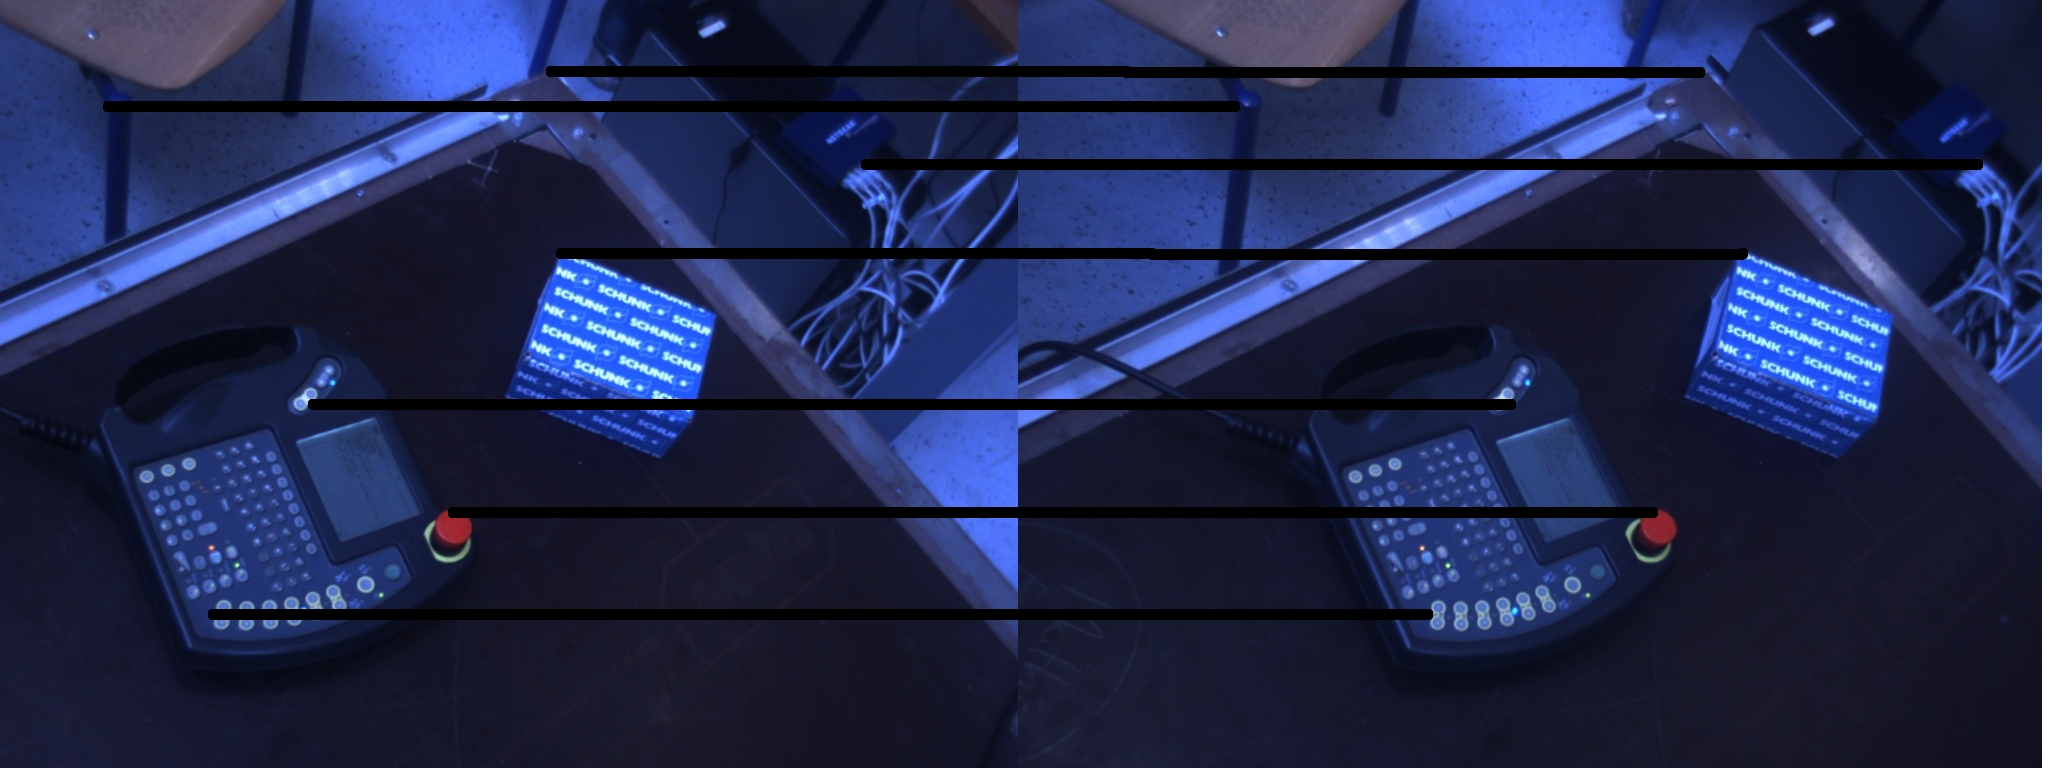
\includegraphics[width=\textwidth]{graphics/06_vision/rectified.jpg}
      \caption{Result of undistortion and rectification on an image pair. The horizontal lines shows corresponding pixels in the two images.}
    \label{fig:rectified}
\end{figure}

\subsection{Disparity map}

From two rectified images the disparity map can be created. Figure \ref{fig:disparity} is an example of such a disparity map. The overall structure of the scene is recognizable, but it can be seen that algorithm does not necessarily guarantees complete coverage with standard parameters. Thus section \ref{sec:optimizing_parameters} will include a discussion of the selection of these parameters.

\begin{figure}[h!]
   \centering
    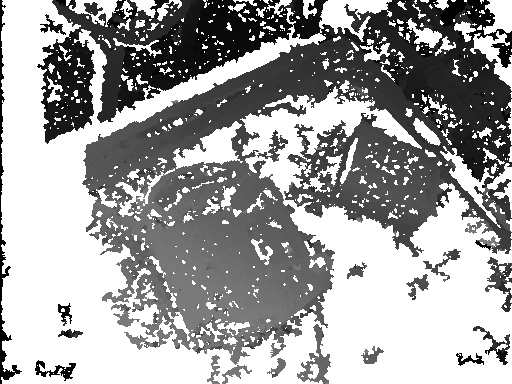
\includegraphics[scale=0.4]{graphics/06_vision/disparity_example.jpg}
    \caption{Disparity image for the two images shown in figure \ref{fig:rectified}. }
    \label{fig:disparity}
\end{figure}


\subsection{Reprojected point clouds} \label{sec:repro_point}

The only thing left to do is reprojecting the disparity map into 3D coordinates. From the calibration the parameters in \ref{eq:parameters} were given for the right camera.

\begin{equation}\label{eq:parameters}
\begin{split}
C_{x} = 582.152313 \\
C_{y} = 393.397633 \\
F_{x} = 1321.556521 \\
-F_{x}T_{x} = 158.751707 
\end{split}
\end{equation} 

Given $ -F_{x}T_{x} $ the baseline between the cameras calculated as in equation \ref{eq:baseline}.

\begin{equation}\label{eq:baseline}
\begin{split}
Tx = -F_{x}T_{x}/(-Fx) = Tx = 158.8/-1321.6 = 0.1201 meters
\end{split}
\end{equation} 

Using these parameters for the Q-matrix, the disparity image is reprojected to 3D. An example of the reprojection for the disparity image in figure \ref{fig:disparity} can be seen in figure \ref{fig:point_repro}


\begin{figure}[h!]
  \centering
    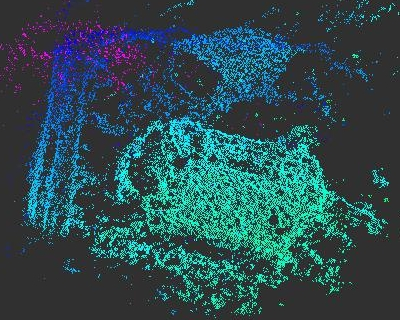
\includegraphics[scale=0.7]{graphics/06_vision/point_cloud_example2.jpg} %trim=l b r t
  \caption{Point cloud reprojected using the parameters shown in section \ref{sec:repro_point} performed on the disparity image in figure \ref{fig:disparity}. }
    \label{fig:point_repro}
\end{figure}


\section{ Optimizing parameters towards the task } \label{sec:optimizing_parameters}

In most of the functions the input were non-adjustable values, but for the SGBM there are certain parameters were no single answers exist. The most important being the disparity range i.e. how far the algorithm will search for disparities.


When the 3D positions were extracted in section \ref{sec:reprojection} the connection in equation \ref{eq:disp1} between distance and disparity were found.

\begin{equation}\label{eq:disp1}
\begin{split}
Z = \dfrac{F_{x}}{ d(-1/T_{x})}
\end{split}
\end{equation} 

When solving for disparity the connection in equation \ref{eq:disp2} is given.

\begin{equation}\label{eq:disp2}
\begin{split}
 d = \dfrac{F_{x}T_{x}}{ Z}
\end{split}
\end{equation} 

That is with a known distance to the setup the one knows the search area, and thus the disparity range can also be calculated. Thus the distance is around 0.5 meters and the focal length and baseline is known from the calibration and shown in section \ref{sec:repro_point}. Thus the expected disparity can be calculated as in equation \ref{eq:disp3}.

\begin{equation}\label{eq:disp3}
\begin{split}
d = \dfrac{1321.55 pixel*0.1201m}{0.5m} = 317.4 pixel
\end{split}
\end{equation}

Thus the minimum and maximum disparity both have to range around this number. It is because of this that the point cloud generated from the ROS $image\_proc$ cannot be used. The node is only able to search with a maximum disparity range of 128 pixel. This gives a minimum distance of 1.24 meters. This wouldn't fit the desired setup at all and therefore the automatically generated point cloud is rejected. The exact disparity range can be found by looking at the maximum size of the object. This is an important aspect as setting the correct disparity range will drastically increase the search time and potentially remove mismatches.

The algorithm is only able to scale the disparity in ranges of 16.

From these equations the minimum and maximum disparity are respectively chosen to be 16*16=256 and                                   16*24=384, resulting in a range from 0.41 to 0.61 meters. Thus if the distance to object should move outside this range it will not be found.

Speckle settings are another important parameter. The speckle-size is the minimum size of a path for it not to be removed as noise and the speckle-range is how large the difference can be between neighbouring pixels for them to still be considered from the same path. Though adjusting this depends entirely on the use of the point cloud. If the reconstruction doesn't take care of noise the speckle-size should be very low. The speckle range should also accommodate the point cloud so as to keep the signal/noise as high as possible, but still fitting the system. 



% Modelling
\chapter{Modelling}
The task of reconstructing an unknown surface from a point cloud is not a trivial task. Especially not when this point cloud is obtained through a camera mounted as the tool on a robot arm. To be able to reconstruct the full surface several views of the object are required, which mean that several point clouds are required to be aligned with each other and stitched together. The modelling component of this system is divided into two sub-components, the first component described in this chapter is filtering and the second component described is the reconstruction component. 

\section{Filtering}
Filtering of raw point clouds is required because of several different reasons. The number of points delivered to the modelling component from the raw point clouds is huge, so filtering non-interesting points away creating a region-of-interest (ROI) in the raw point clouds. Lowering the number points in each cloud delivered to the modelling component is required such the workload can be kept within an acceptable range. The number of points can be further reduced by down-sampling the points left in the ROI by the cut-off filter. A voxel-grid filter utilised for down-sampling also creates the advantage of equal sampling density, but the disadvantage is that the down-sampling means loss of information, and therefore there is a trade off between speed and level of detail of the reconstruction process.  

\begin{figure}[htb]
	\begin{center}
		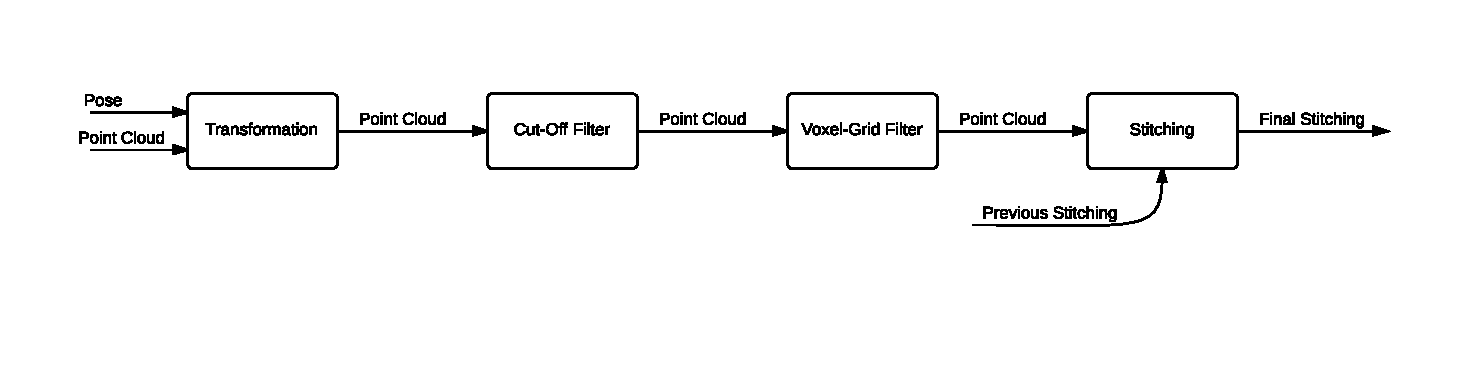
\includegraphics[scale=0.6,trim=20 70 0 20]{graphics/07_modelling/FilterFlow.pdf}%trim=l b r t
		\caption{Illustrates the flow through the filter.}
		\label{fig:filter_flow}
	\end{center}
\end{figure}

In figure \ref{fig:filter_flow} an illustration of the flow through the filter can be seen. The vision layer is delivering a point cloud for each individual view, along with this point cloud a pose of the frame in which the points are recorded is delivered. These two sets of data is delivered to the ROS node which handles filtering, this node filters each individual cloud and stitches each of them together in a common cloud. This common cloud, when finished, is sent to the reconstruction layer. In the sections below is a brief description of the components shown in figure \ref{fig:filter_flow}. 

\subsection{Point cloud library}
The Point Cloud Library (PCL) utilised in this project is a library which provide functionality for working on 3D point clouds. PCL delivers a variety of functionality such as filters, segmentation, surface reconstruction, kd- and oc-trees, visualisation, etc. PCL can be found at http://www.pointclouds.org/, along with documentation and tutorials.

\subsection{Point cloud transformation}
Messages received from the vision layer needs to be processed before filtering. This is because the messages delivered to the modelling component contain a point cloud and a pose of the current camera view. The coordinates of the individual points in the cloud are related to the camera frame, but this frame is moving around the object so a transformation of points is needed such they can be related a common static frame.

\begin{figure}[htb]
	\begin{center}
		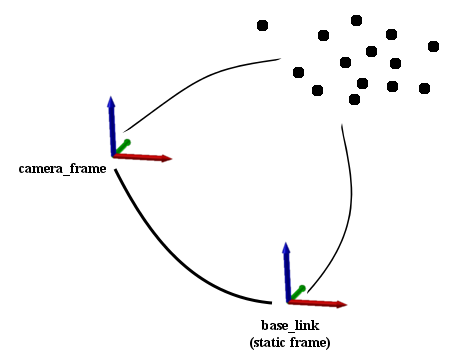
\includegraphics[scale=0.7,trim=0 0 0 0]{graphics/07_modelling/pctransform.png}%trim=l b r t
		\caption{Illustrates points in different frames.}
		\label{fig:filtering_transform}
	\end{center}
\end{figure}

\subsection{Cut-off filter}
The cut-off filter utilised is the implementation from PCL, \texttt{pcl::PassThrough< \ldots >}. A cut-off filter is utilised to create a ROI in the transformed point cloud, partly because the number of points needs to be reduced with respect to processing time and then because the region in which the object resides is fairly small to the region which is recorded by the camera.

\subsection{Voxel-grid filter}
The voxel-grid down-samples the left overs from the cut-off filtering. The down-sampling causes loss of information which mean that surface details are lost in the process, so the amount of down-sampling should be chosen with respect to processing time versus level of detail to be reconstructed. The PCL library luckily have such functionality (\texttt{pcl::VoxelGrid< \ldots >}) which is utilised in the filtering sub-component.\\
\\
The voxel-grid filter works by splitting down the ROI into smaller regions (voxels) of certain resolution in which each of the voxels are analysed. Figure \ref{fig:filtering_voxel_grid} show the principle of the voxel-grid. A new point is approximated for each voxel, the new point is approximated by the points centroid which is contained in the voxel. This method is a little slower compared to just placing the new point in the center of the voxel, but it helps save some more detailed information about the surface curvature.
\begin{figure}[htb]
	\begin{center}
		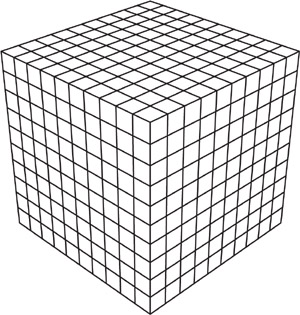
\includegraphics[scale=0.7,trim=0 0 0 0]{graphics/07_modelling/cube.jpg}%trim=l b r t
		\caption{Illustrates a cube consisting of 10x10x10 cubes which resembles the voxel-grid filter.}
		\label{fig:filtering_voxel_grid}
	\end{center}
\end{figure}

\subsection{Point cloud stitching}
\marginnote{Subsection not finished}

The individual point clouds from the individual views of the object are passed through the filter, the individual cloud is then stitched into another common cloud which is assembled from a number of individual clouds, predetermined by the decision making layer. The stitching of each cloud happens in the static frame, due to the transformation of the input to the filter node. The point clouds are stitched in the order at which they are received, thus the first frame becomes a sort of reference frame for the following frames. This is because the algorithm used for stitching the clouds together actually calculates a transform at which new incoming point clouds are transformed. The algorithm utilised for stitching is Iterative Closest Point (ICP). This is also implemented in in PCL and therefore this implementation (\texttt{pcl::IterativeClosestPointNonLinear< \ldots , \ldots >}) of the algorithm utilised. The ICP algorithm has it downsides. For example if a cloud is not aligned correctly, this will cause an error to propagate thought to the following clouds which could lead to a rather distorted model of the object of interest\cite{choe2007registration}. The algorithm will be described in further details in chapter \texttt{ref??}\marginnote{Ref til calibration chapter}.
\section{Surface reconstruction}
Surface reconstruction from a large set of unstructured points obtained through laser scanning techniques or stereopsis is not a trivial task but nonetheless it is useful in many applications. For example a surface reconstruction could aid a robots end effector grasping some unknown object \cite{Wang2005}. Many methods for surface reconstruction exist in different domains of science, some algorithms are based on neural network approaches  \cite{Wu2007}, others are based on sculpting or region growing algorithms (e.g \cite{Bernardini1999} and \cite{Amenta2001}) used in computational geometry, some utilise an implicit method framework to represent incoming data as a surface \cite{Kazhdan2006} and \cite{Dong2011}.\\
\\
In 1999 F. Bernardini \textit{et al}. proposed in a fairly simple algorithm (Ball Pivoting Algorithm (BPA)) for reconstruction of surfaces from point clouds sampled over smooth objects \cite{Bernardini1999}. BPA is pivoting a sphere of a certain diameter around an edge of a seed triangle. Pivoting the sphere around all the edges is connecting three points to form a new triangle and so on. BPA is a part of the region growing algorithms as this algorithm uses a seed triangle builds the surface around this and outward. The algorithm is fairly easy to work with as it has one parameter which decides the radius of the sphere and that is it. N. Amenta \textit{et al}. proposed in 2001 \cite{Amenta2001} the power crust algorithm, which essentially is a three dimensional Voronoi approach \cite{Ledoux2007}. The power crust algorithm is well defined and proven which makes it one of the most known algorithm regarding surface reconstruction. This algorithm is a sculpting algorithm in computational geometry. Common for those algorithms mentioned is that these are explicit methods which requires neighboring information which leads to high computational time consumption. Therefore methods mentioned above are not well suited for reconstruction of large data sets.\\
\\
In 2006, M. Kazhdan \textit{et al}. proposed in \cite{Kazhdan2006} an algorithm which resides in the implicit method framework, this algorithm is called Poisson Surface Reconstruction (PSR). PSR is a fitting scheme that allow solving for the indicator function of the surface. It is shown in \cite{Kazhdan2006} this approach of fitting a surface resembles the Fast Fourier Transform (FFT). In \cite{Kazhdan2006} it is shown that the FFT approach requires five times as much space but is approximately double as fast while creating approximately the same number of triangles. The real advantage of the Poisson approach is that it is scalable and therefore does not rely on a uniform distribution of points and thus a higher degree of details can be reconstructed in areas where the point density is higher.\\
J. Manson \textit{et al}. did in 2008 propose a wavelet approach of the problem of reconstructing surfaces of large sets of unstructured points \cite{Manson2008}. The method is robust to noise in data because it is relying on implicit methods as PSR, and is therefore well-suited for reconstruction of real data which is overlayed with some random noise. The wavelet approach an advantages over PSR, the wavelet approach is able to reconstruct non-closed surfaces in opposition to PSR \cite{Kazhdan2006}. Using the Haar wavelet synthesise an acceptable surface if the points are well-aligned, else more smooth wavelets can be used such as Daubechies-2. Using octrees and small-support wavelets makes the synthesisation very fast, smaller support equals less computational time and space. Using Daubechies-2 compared to Haar increases computational time by a scale of four, and the space consumption is upscale by approximately four as well. As the methods for reconstruction mentioned first does not guarantee watertight mesh and does not work very well with large point sets, mean those methods are not of interest for further studies. The PSR and the wavelet approach both does estimate an indicator function of the surface, but each handles this indicator function differently. As these method is based on implicit methods they are more robust to noise in the input and approximates the surfaces better compared to the methods mentioned first.

\subsection{Overview of reconstruction scheme}
The wavelet method for surface reconstruction chosen for this custom implementation is highly inspired by the description in \cite{Manson2008}. One main reason for using wavelets for the analysis of the surface compared to more conventional methods like FFT is that wavelets support localisation in spatial and frequency(scale) domains. This mean that analysis is made locally instead of globally, which leads to the possibility of reconstructing finer details in input data, that would otherwise be hidden by the global analysis. PSR is approximating an indicator function\marginnote{ref: indicator function} of the surface by solving a Poisson equation\marginnote{ref: Poisson eq.}. In the wavelet approach an indicator function is also estimated, but the way it is done is different. The wavelet approach approximates the wavelet coefficients of the indicator function by making a multi resolution analysis (MRA) of the input data\marginnote{ref: MRA, coeffs}. After the coefficients have been calculated ...

\subsection{Indicator function}
The method mentioned in \cite{Manson2008} defines the indicator function of the surface $\partial M$ of an object $M$ to be as follows

\begin{equation}
	\chi_M(\textbf{x}) =  
	\label{eq:indicator_fnc}
\end{equation}



\begin{equation}
	c^e_{j,\textbf{k}} \approx 2^{3j \over 2} \sum_{p_i \in \partial M \cap \textit{supp}(\psi^e_{j,\textbf{k}})} \vec{F}^e_{j,\textbf{k}} (p_i) \cdot \vec{n}_i d \sigma_i 
	\label{eq:wavelet_coeffs}
\end{equation}

\subsection{Mesh generation}

\subsection{Implementation}
The surface reconstruction is implemented in ROS node making it compatible with the rest of the system. The assembled point cloud is passed from the filter node to the reconstruction node. PCL is used for estimating normals of the points in the assembled point cloud. 

\subsection{Results}

% Calibration
\chapter{Calibration}
In the process of combining data from several view points, a model of the system is needed as to align the measurements correctly. An idealised model can be formulated based on motion theory, but in inherently imperfect hence the need for calibration. In the context of eye-in-hand based surface reconstruction, especially calibrating the kinematic chain from object robot base is important in order to combine data from several views. Calibration of robot systems has received considerable attention and continues to be an active field of research. A solution for the unknown transforms from camera to end effector and from object to robot base can be obtained relatively easy by solving a homogeneous transform \cite{Shiu1989}. Several algorithms for more or less autonomous calibration has been proposed \cite{Tsai1988, Tsai1989} often simultaneously calibrating camera and hand-eye \cite{Malm2003, Zhao2008, Jordt2009}. The calibration process presented here is based on the linear method \cite{Tsai1988} with some application specific modifications.


\subsection{Notation}
In the formulation of hand-eye calibration a number of homogeneous transforms between frames are be described. Most literature uses a mathematically founded notation of \textit{Ai}, \textit{Bi}, \textit{A}, \textit{B}, \textit{X} and \textit{Y} leading to nice and clean equations. In this work a more explicit and engineering friendly notation will be used stating for each transform the state index (since there are several different robot states involved to allow different views of the object), the name of the frame described and the name of the reference frame. Examples of the notation are explained in table \ref{tab:notation}. The transform is a a 4x4 matrix containing a 3x3 rotation matrix and a 1x3 translation vector. The terms end-effector and Tool Center Point(TCP) will be used interchangeably.\\

\begin{table}[h]
\caption{Examples of the notation used to describe rigid transformation.}
\begin{tabular}{ll}
\label{tab:notation}
$[T_{i}]_{camera}^{object}$   & The transform from object to camera at the \textit{i}th robot state          \\[8pt] 
$[T_{i}]_{base}^{TCP}$        & The transform from end-effector to base at the \textit{i}th robot state      \\[8pt] 
$[T_{i}]_{TCP}^{camera}$      & The transform from camera to end-effector at the \textit{i}th robot state     \\[8pt] 
$[T_{i-1,i}]_{camera}$        & The camera frame at state \textit{i} relative to the camera frame at state \textit{i-1}  \\[8pt]              
\end{tabular}
\end{table}

\begin{figure}[htb]
	\begin{center}
		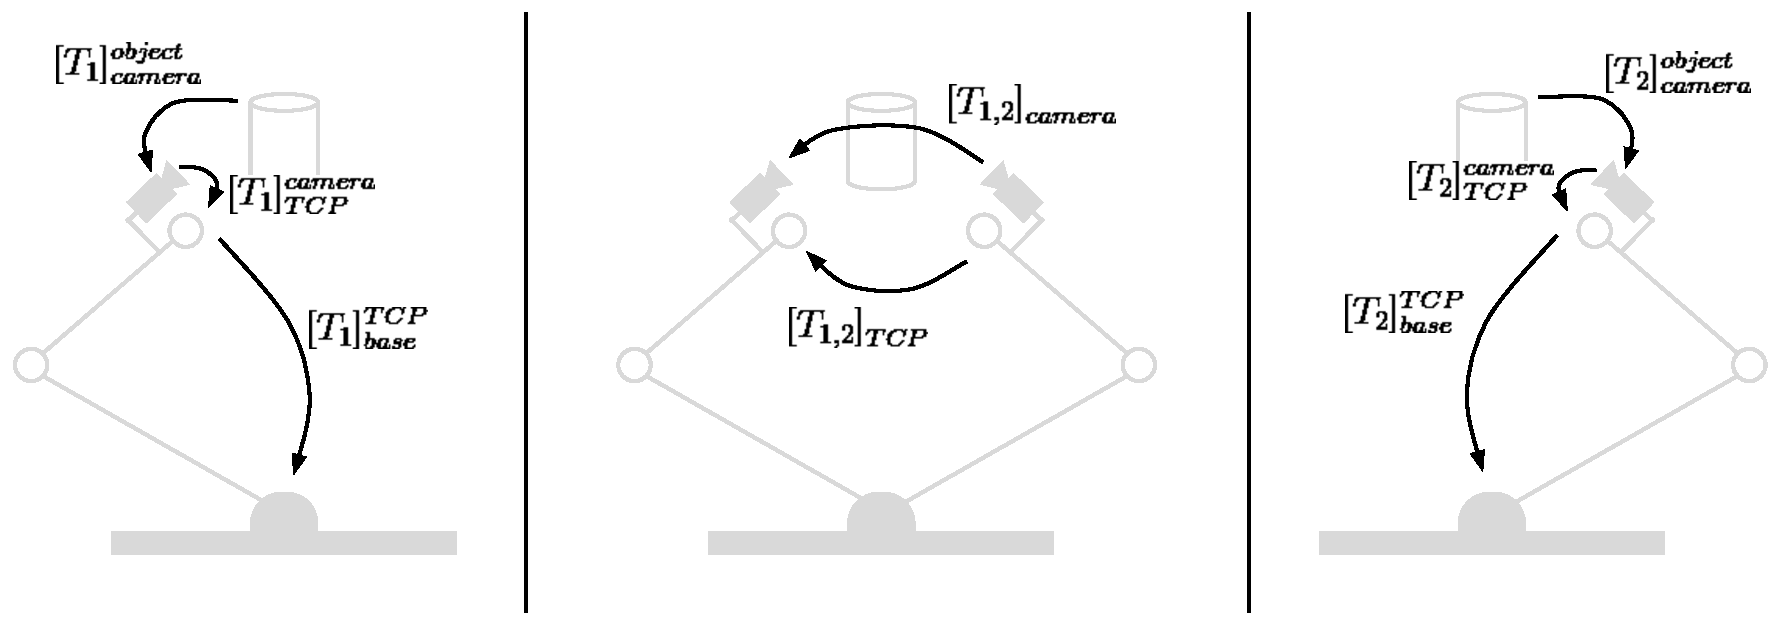
\includegraphics[width=\textwidth,trim=0 0 0 0]{graphics/03_calibration/hand_eye_transforms.pdf}%trim=l b r t
		\caption{Sketch of a robot with a camera mounted on the end-effector in two different states capturing a cylinder object. Shows the robot in state 1 (left), state 2 (right) and both robot states in same image (center).}\label{fig:hand_eye_transforms}
		
	\end{center}
\end{figure}

\subsection{Linear hand-eye calibration}
\noindent Looking at figure \ref{fig:hand_eye_transforms} (left and right) it is clear that a kinematic chain from the object to the robot base can be formulated.\\

\begin{equation}
	[T_{i}]_{base}^{object} = [T_{i}]_{base}^{TCP} \cdot [T_{i}]_{TCP}^{camera} \cdot [T_{i}]_{camera}^{object}
\end{equation} \\

\noindent The transform from end-effector to robot base can be found from the joint states of the robot and the transform from object to camera can, assuming the camera is calibrated, be found from projection geometry. This leaves only the transform from camera to end-effector as unknown. Assuming that the object is static and captured from different robot states, it is possible to formulate the transform between the two camera poses (Figure \ref{fig:hand_eye_transforms}, center).\\

\begin{equation}\label{eq:object_camera}
\begin{matrix}
[T_{1,2}]_{camera} \cdot [T_{1}]_{camera}^{object} = [T_{2}]_{camera}^{object} \\
\\  
\Updownarrow \\ 
\\ 
[T_{1,2}]_{camera} = [T_{2}]_{camera}^{object} \cdot ([T_{1}]_{camera}^{object})^{-1}
\end{matrix}
\end{equation}\\ 

\noindent Similarly the transform between the two poses of the end-effector can be formulated(\ref{fig:hand_eye_transforms}, center).\\

\begin{equation}
\begin{matrix}
[T_{1}]_{base}^{TCP} \cdot [T_{1,2}]_{TCP} = [T_{2}]_{base}^{TCP} \\ 
\\ 
\Updownarrow \\ 
\\ 
[T_{1,2}]_{TCP} = ([T_{2}]_{base}^{TCP})^{-1} \cdot  [T_{1}]_{base}^{TCP}
\end{matrix}
\end{equation}\\ 

\noindent Assuming that the transform from camera to end-effector is static it is clear that.\\

\begin{equation}
[T_{1}]_{TCP}^{camera} = [T_{2}]_{TCP}^{camera} = [T]_{TCP}^{camera}
\end{equation}\\ 

\noindent This makes it possible to formulate a closed loop kinematic chain (\ref{fig:hand_eye_transforms}, center). This equation is in most literature denoted $ AX=XB $. \\

\begin{equation} \label{equ:closed_loop}
	[T_{1,2}]_{camera} \cdot [T]_{TCP}^{camera} = [T]_{TCP}^{camera} \cdot [T_{1,2}]_{TCP}
\end{equation}\\ 

\noindent The missing transform can thus be found by solving a set of $ n-1 $ linear equations for $ n $ robot states \\

\begin{equation} \label{eq:linear_equations}
\left\{\begin{matrix}
[T_{1,2}]_{camera} \cdot [T]_{TCP}^{camera} = [T]_{TCP}^{camera} \cdot [T_{1,2}]_{TCP} \\ 
\ \ \vdots 
\\ 
[T_{i-1,i}]_{camera} \cdot [T]_{TCP}^{camera} = [T]_{TCP}^{camera} \cdot [T_{i-1,i}]_{TCP}\\ 
\ \ \vdots 
\\ 
[T_{n-1,n}]_{camera} \cdot [T]_{TCP}^{camera} = [T]_{TCP}^{camera} \cdot [T_{n-1,n}]_{TCP}
\end{matrix}\right.
\end{equation}\\ 

\noindent Normally the calibration is made by capturing views of a chessboard marker from several robot states. There are however two rather implicit assumptions \cite{Horaud1995} not justified by this approach. First the calibration of the camera assumes a perfect pinhole model and that the optical axis of the camera is perpendicular to the object, but equation \ref{equ:closed_loop} assumes that the object is static, which for most practical objects are contradictions. There are several approaches to solving this, but those are outside the scope of this discussion. 

\marginnote{Refs} 

\subsection{Application specific method}
In this work an alternative approach is taken to include more of the possible uncertainties in the hand-eye calibration and to account for the unjustified assumptions mentioned above. Uncertainties in the vision process generating the transform from object to camera could stem from inaccurate parameters, the pinhole model assumption or pixel quantisation errors to mention a few. Uncertainties in the transform from end-effector to base can stem from mechanical inaccuracies, wear and tear, quantisation errors in encoders or from dynamics, also just to mention a few. \\

\noindent Solving the linear system from equation \ref{eq:linear_equations} is equivalent to making a least-squares fit and thus after calibration a fixed transform minimising the error over all robot states is applied to each state. The problem with this is that a linear method is used to estimate errors that are by no means linear. Furthermore the method is vulnerable to outliers, since one faulty view will influence all others. Instead a method capable of fitting non-linear functions is desirable, but to use such, individual errors at each robot state must be known. Furthermore it is desired to include as much of the reconstruction process as possible inside the the calibration loop, to account for as many errors as possible. Therefore it is desirable to base the calibration on the point clouds instead of the camera output and furthermore it is desirable to evaluate each data pair instead of pooling them for all views.\\

\noindent Estimating a rigid transform between two point clouds is considered an absolute orientation problem \cite{Horn1987} and can be solved with an Iterative Closest Point(ICP) algorithm. The ICP algorithm tries to estimate a transform to align the source cloud to the target cloud by alternating between matching points that are close, estimating the transform and transforming the remaining points. Normally the transform is estimated using least-squares, but an alternative implementation using damped least-squares\cite{Gavin2011} and thus not assuming linearity is found in PCL (\texttt{pcl::IterativeClosestPointNonLinear< \ldots , \ldots >}). This is already implemented as part of the point cloud registration process is the modelling component where it is used for pairwise alignment of the point clouds as part of the registration process. Knowing the pairwise pose estimate means that another closed loop formulation can be expressed (Figure \ref{fig:new_calibration}). \\

\noindent Taking as example the camera pose at state 1 ($ [T_1]_{base}^{camera} $) and following the pairwise alignment transforms all the way around ending up back at state 1 the result must be equal to the original pose and the error at that pose.

\begin{equation}
\begin{matrix}
[T_{1}]_{base}^{camera} \cdot [T_{12}]_{PC} \cdot [T_{23}]_{PC} \cdot [T_{34}]_{PC} \cdot [T_{45}]_{PC} \cdot [T_{51}]_{PC} = [T_{1}]_{base}^{camera} \cdot [T_{1}]_{camera}^{error}
\\ 
\Updownarrow \\ 
\\ 
[T_{12}]_{PC} \cdot [T_{23}]_{PC} \cdot [T_{34}]_{PC} \cdot [T_{45}]_{PC} \cdot [T_{51}]_{PC} = [T_{1}]_{camera}^{error}
\end{matrix}
\end{equation}\\ 

\noindent Looking at the closed loop in figure \ref{fig:new_calibration} if say the view at state 3 had a large error, that error would in the evaluation of all other states result in two contributions ($ T_{23} $ and $ T_{34} $) of equal magnitude and opposite sign. This means the method is robust to outliers. Now having estimated the error at each pose, a non-linear method can be used to estimate the calibrated transform. The ideal method would be one eliminating the error in each state, while interpolating in between. However such a method cannot be made with a static transform.

\marginnote{Her er der som jeg ser det to muligheder. Enten følger vi Kents idé om at publicere et dynamisk tf som interpolerer mellem fejlene eller også benytter vi en damped least-squares eller lignende til at bestemme et statisk tf...}

\begin{figure}[htb]
	\begin{center}
		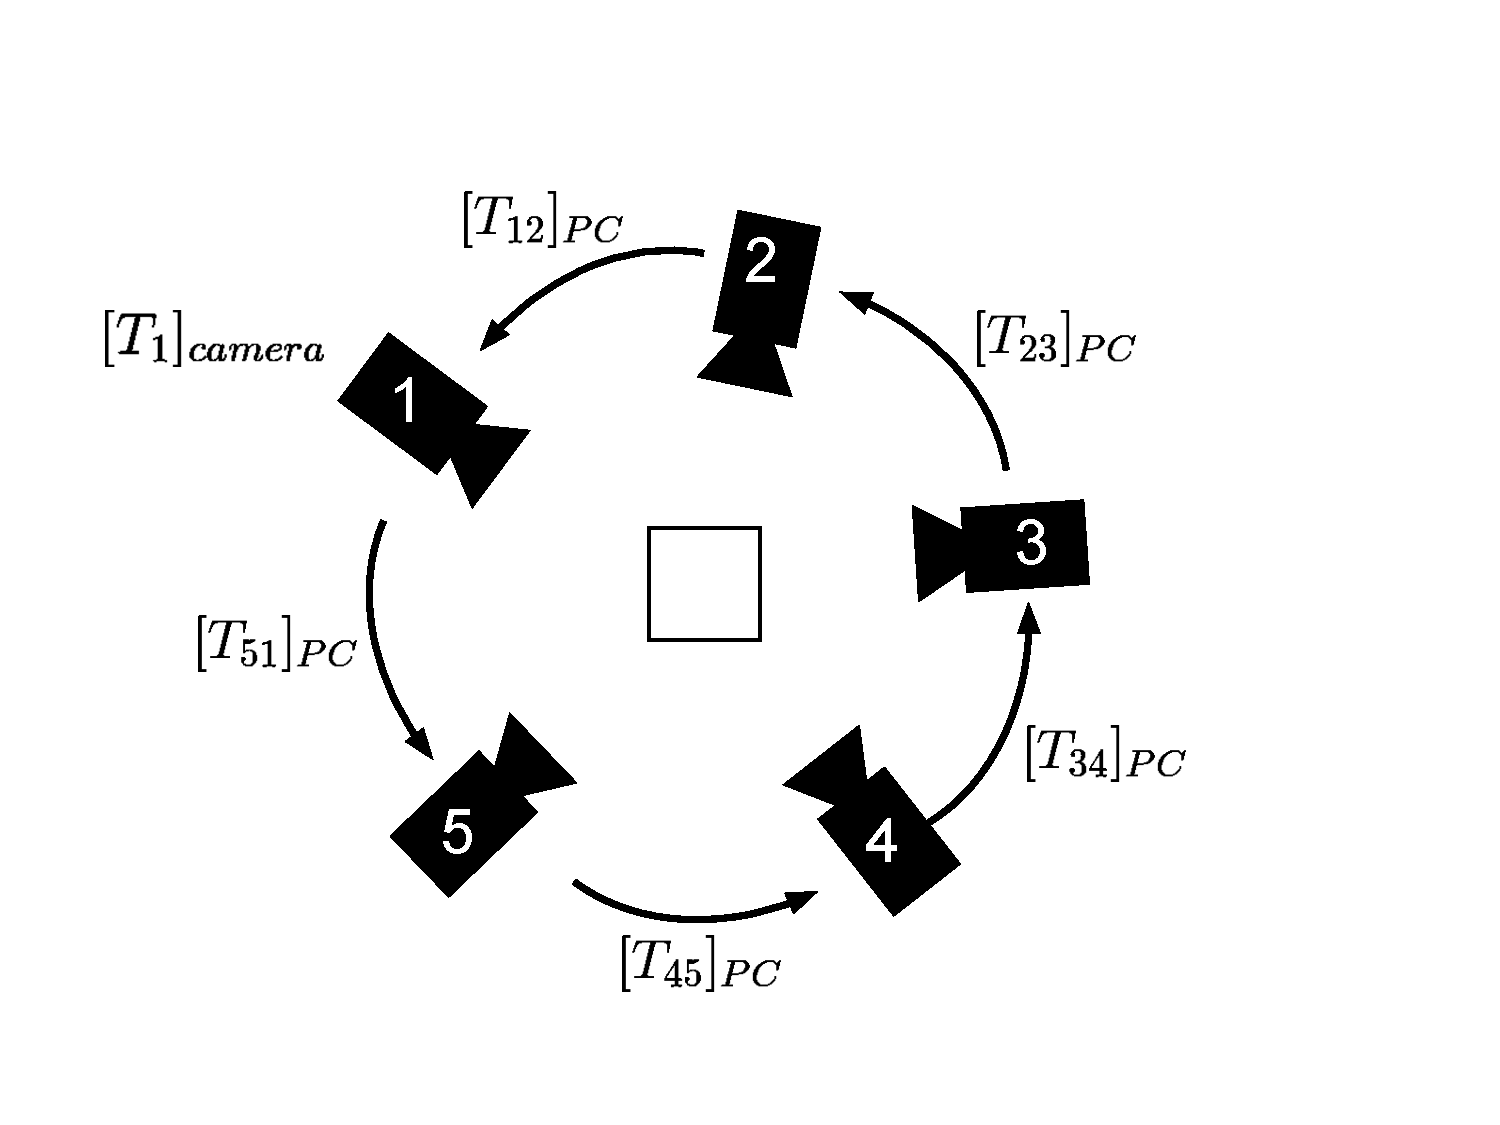
\includegraphics[scale=0.4,trim=0 0 0 0]{graphics/03_calibration/new_calibration.pdf}%trim=l b r t
		\caption{The closed loop formed by the point cloud transformations.}\label{fig:new_calibration}
	\end{center}
\end{figure}


 





% Results andwill  discussion
\chapter{Preliminary Results}
Evaluation of the system is based on a comparison between the hand-eye calibration module implemented in ROS and the proposed application specific calibration. Although several experiments were made, they mostly served to get acquainted with the system and the results are insufficient to draw any final conclusions. In the following the observations will be presented and discussed.\\

The experiments consisted of running the system approximately 20 times varying the object, density of views, parameters on the camera, parameters on the carmine sensor, lighting conditions, stitching parameters, classic hand-eye calibration, the proposed method for calibrations etc. In all cases the performance of the system was poor and thus quantitative comparison to the original model was omitted. \\

Comparing the hand-eye calibration implemented in ROS to the proposed system failed because both systems produced very inconsistent transforms.\\

\section{Calibration transforms}
Some of the results from the proposed calibration method are listed here. The calibration transform is kept in the aerospace convention such roll, pitch and yaw, resembling the euler angles around x-, y- and z-axis respectively. 

% Conclusion
\chapter{Discussion}
Although the results were insufficient to draw any final conclusions, some of the many observations and reflections are worth mentioning. Many factors and decisions has influenced the project both good and bad and therefore also deserves discussion to draw experiences.\\

There has been many advantages from implementing the entire system in ROS leading to significantly reduced development time. The rosbag tool made it possible to work offline and thus enabled parallel development of components and effectiveness despite limited access to the robot. Being able to facilitate the rviz visualisation tool provided a safe and intuitive control, since the pinhole of the camera could be placed at will. ROS also delivered increased flexibility because of close integration with many state of the art libraries and frameworks as well as support for both python and C++ programming languages. The architecture of the designed system combined with the inter process communication model provided in ROS made the interfaces clear and further enhanced effective work. Finally the vast communities of ROS, OpenCV, PCL, OMPL etc. has been invaluable.\\

There have been many challenges in the project and many of them influenced its outcome. First there were great challenges with the reach of the robot compared to the range of the sensors. Even when the object was hanged from a point above the robot, the maximum radius of the sphere was 45cm with is close to the 40cm minimal range of the carmine sensor and leading to a very large disparity of 130 on the bumblebee camera. This challenged the rectification process, increased noise on the point cloud and thus also challenged the stitching process. Hanging the object also introduced the problem of fixing the object because the work cell fence is not fixed and thus the slightest touch would make the object swing again challenging the system.\\

During experimentation it became very apparent that some implicit assumptions had been made and those made even simple tasks very difficult. As mentioned above, it was implicitly assumed that everything would be static during capture, which is never a problem when working on the Canterbury images, but is a great problem in reality. The disparity in the Canterbury set is usually around 16 and this was implicitly assumed to be the case however it turned out to be almost twenty times as large. The list is much longer but a point has been made, that even though having focused on requirements and assumptions all along, important issues were hidden from the beginning due to inexperience.\\

The vision features turned out to be a much greater challenge than expected. Even with good lighting, unique features on the object and a calibrated system, the quality of the point clouds were still too poor to do 3D reconstruction on, which underlines another implicit assumption, that reconstruction is at all possible in this set up. Although much better with the active Carmine sensor, the point clouds were still somewhat poor, and by no means matched the quality of point clouds that are presented in papers, textbooks and programming examples. The importance of features in the point cloud and the importance of sufficient overlap also became evident as did the profound differences between active and passive sensing.\\

The proposed calibration method performed as a proof of concept, although exhibiting the effects of many of the implicit assumptions. The performance in the present experiments were poor, but given the right application and further advances in pose estimation of noisy point clouds, it might hold potential. The system in general, but calibration in particular performed too poor to be evaluated in the manner planned based on comparison between point cloud and 3D model.\\

\chapter{Conclusion}
Even if a clear conclusion cannot be made at this point about the stated hypothesis, some partial conclusions can be made. The calibration method worked, but performed poorly and can thus not be recommended at this point. The implementation of the system in ROS based on the environment interaction model worked well. \\


\section{Learned lessons}
Probably the most important lessons learned in this project is humility to the level of complexity in the proposed system and to the process of developing a complete system as first time experience with practical robotics. So many things have been a first encounter from simple online/offline considerations to working with real noisy data. In many cases idealised small-scale experiences comprised the origin for decisions about a very real full-scale robotics system making an example of the vast differences between two worlds.


% References
\clearpage
\nocite{*} % Includes all of the .bib content
\printbibliography\addcontentsline{toc}{chapter}{Bibliography}

% Appendix
%\appendix %all sections below are numbered A, B, C,...
%\chapter{Sample appendix}
RoVi is the best course ever .... blablabla



\end{document}
